\documentclass[a4paper,12pt]{book}
\usepackage{graphicx}
\usepackage[export]{adjustbox}
\usepackage{subcaption}
\graphicspath{{Pics/}}
\usepackage{charter}
\usepackage{fancyhdr}
\usepackage{enumerate}
\usepackage{enumitem}
\usepackage{siunitx}
\usepackage{amssymb}
\usepackage{longtable}
\usepackage{multicol}
\usepackage{multirow}
\usepackage{hhline}
\usepackage{parskip}
\setlength{\parskip}{6pt}
\usepackage{ragged2e}
\usepackage{geometry} %margin
\geometry{left=2.1cm,right=2.1cm,top=3cm,bottom=3cm}
\usepackage{setspace}
\SetSinglespace{1.2}
\singlespacing
\renewcommand{\ttfamily}{\fontfamily{pcr}\selectfont}
%\renewcommand{\familydefault}{\rmdefault}

\usepackage[,table]{xcolor}
\definecolor{LightBlue}{cmyk}{0.16,0.03,0.04,0}
\definecolor{Title}{cmyk}{0.8,0.1,0,0.3}
\setlength{\arrayrulewidth}{0.3mm}
\setlength{\tabcolsep}{2pt}
\setlength{\headheight}{15pt}
\renewcommand{\arraystretch}{1}
\usepackage{tikz}
\usepackage{nicematrix}
\newcommand*\circled[1]{\tikz[baseline=(char.base)]{\node[shape=circle,draw,inner sep=1pt] (char) {#1};}}

\newcolumntype{s}{>{\columncolor{Title}\RaggedLeft} m{3.5em}} % columntype for chapter title
\newcolumntype{d}{>{\columncolor{LightBlue}\RaggedRight} m{\textwidth}} % columntype for code bloc
\newcolumntype{a}{>{\columncolor{LightBlue}\RaggedRight} m{0.96\textwidth}} % columntype for secondary code bloc

\usepackage{titlesec}
\usepackage[hidelinks]{hyperref}
\urlstyle{same}

\captionsetup[figure]{labelsep=period,font={bf}}
\captionsetup[table]{font={bf},labelsep=period}

\newcommand{\titlename}{}

\newcommand{\chaptertitle}[2]{ %reset chapter format
\vspace{-120pt}
\gdef\titlename{#1}
{
\SetSinglespace{1.1}
\singlespacing
\Huge\bfseries
\setlength{\tabcolsep}{8pt}
\renewcommand{\arraystretch}{1.5}
\begin{tabular}{s >{\RaggedRight}m{14.5em}}
\textcolor{white}{Chapter\newline\thechapter}&\textcolor{Title}{#2}
\end{tabular}
}
}

\newcommand{\partpic}[1]{%insert picture
    \tikz[remember picture,overlay] \node at (current page.center){\includegraphics[width=\paperwidth]{#1}};
}

\titleformat{\part} %reset part %format
{\huge\bfseries} % format
{} % label
{0em} % sep
{\Centering} % before-code

\titleformat{\chapter} %reset chapter %format
{\huge\bfseries} % format
{} % label
{0em} % sep
{\Centering} % before-code
\titlespacing{\chapter}{0pt}{0pt}{0pt}

\titleformat{\section} %reset section %format
{\Large\bfseries} % format
{\textcolor{Title}{\thesection}} % label
{0.5em} % sep
{\color{Title}} % before-code
\titlespacing{\section}{0pt}{12pt}{6pt}

\titleformat{\subsection} %reset subsection %format
{\large\bfseries} % format
{\textcolor{Title}{\thesubsection}} % label
{0.5em} % sep
{\color{Title}} % before-code
\titlespacing{\subsection}{0pt}{8pt}{6pt}

\newenvironment{term}[1]{
    \textbf{#1}

    \leftskip 1em
    \parskip 0pt
}

\newenvironment{secterm}[1]{
    \textbf{#1}

    \leftskip 2em
    \parskip 0pt
}

\newenvironment{codebloc}{ %define code bloc style
    \ttfamily\footnotesize
    \renewcommand{\arraystretch}{1}
}

\newcommand{\note}[2][NOTE]{ %Note/Tips
\vspace{6pt}
\begin{tabular}{b{\textwidth}}
\hline
\fontfamily{phv}\selectfont \textbf{#1}\\
\leftskip 1em #2\\
\hline
\end{tabular}
}

\newcommand{\secnote}[2][NOTE]{ %Note/Tips
\vspace{6pt}
\begin{tabular}{b{0.93\textwidth}}
\hline
\fontfamily{phv}\selectfont \textbf{#1}\\
\leftskip 1em #2\\
\hline
\end{tabular}
}

\title{ESP32-C3 Wireless Adventure\par \Large A comprehensive guide to IoT}
\author{Espressif Systems}
\date{\today}

\pagestyle{fancy} % reset head&foot
\fancyhead{} % clear all header fields
\renewcommand\headrulewidth{0pt}
\fancyfoot{} % clear all footer fields
\setcounter{chapter}{1}

\begin{document}

\fancyfoot[LE]{\fontfamily{cmss}\selectfont{\textbf{\thepage} \ \textit{ESP32-C3 Wireless Adventure: A comprehensive guide to IoT}}}
\fancyfoot[RO]{\fontfamily{cmss}\selectfont{\textit{Chapter \thechapter. \titlename} \ \textbf{\thepage}}}

\chapter[Introduction and Practice of IoT Projects]{\chaptertitle{Introduction and Practice of IoT Projects}{Introduction and Practice of IoT Projects}}

\vspace{24pt}
In Chapter 1, we introduced the architecture of IoT, and the roles and interrelationships of the perception \& control layer, network layer, platform layer, and application layer, as well as the development of smart home. However, just like when we learn to paint, knowing the theoretical knowledge is far from enough. We have to “get our hands dirty” to put IoT projects into practice in order to truly master the technology. In addition, when a project moves to the mass production stage, it is necessary to consider more factors such as network connection, configuration, IoT cloud platform interaction, firmware management and updates, mass production management, and security configuration.

So, what do we need to pay attention to when developing a complete IoT project?

In Chapter 1, we mentioned that smart home is one of the most common IoT application scenarios, and smart lights are one of the most basic and practical appliances, which can be used in homes, hotels, gyms, hospitals, etc. Therefore, in this book, we will take the construction of a smart light project as the starting point, explain its components and features, and provide guidance on project development. We hope that you can draw inferences from this case to create more IoT applications.

\section{Introduction to Typical IoT Projects}
In terms of development, basic functional modules of IoT projects can be classified into software and hardware development of IoT devices, client application development, and IoT cloud platform development. It is important to clarify the basic functional modules, which will be further described in this section.

\subsection{Basic Modules for Common IoT Devices}
Software and hardware development of IoT devices include the following basic modules:

\begin{term}{Data collection}
    As the bottom layer of the IoT architecture, the IoT devices of the perception \& control layer connect sensors and devices through their chips and peripherals to achieve data collection and operation control.
\end{term}

\vspace{12pt}
\begin{term}{Account binding and initial configuration}
    For most IoT devices, account binding and initial configuration are completed in one operational process, for example, connecting devices with users by configuring Wi-Fi network.
\end{term}

\begin{term}{Interaction with IoT cloud platforms}
    To monitor and control IoT devices, it is also necessary to connect them to IoT cloud platforms, in order to give commands and report status through interaction between each other.
\end{term}

\begin{term}{Device control}
    When connected with IoT cloud platforms, devices can communicate with the cloud and be registered, bound, or controlled. Users can query product status and carry out other operations on the smartphone app through IoT cloud platforms or local communication protocols.
\end{term}

\begin{term}{Firmware upgrade}
    IoT devices can also achieve firmware upgrade based on manufacturers’ needs. By receiving commands sent by the cloud, firmware upgrade and version management will be realized. With this firmware upgrade feature, you can continuously enhance the functions of IoT devices, fix defects, and improve user experience.
\end{term}

\subsection{Basic Modules of Client Applications}
Client applications (e.g., smartphone apps) mainly include the following basic modules:

\begin{term}{Account system and authorisation}
    It supports account and device authorisation.
\end{term}

\begin{term}{Device control}
    Smartphone apps are usually equipped with controlling functions. Users can easily connect to IoT devices, and manage them anytime, anywhere through smartphone apps. In a real-world smart home, devices are mostly controlled through smartphone apps, which not only enables intelligent management of devices, but also saves the cost of manpower. Therefore, device control is a must for client applications, such as device function attribute control, scene control, scheduling, remote control, device linkage, etc. Smart home users can also customise scenes according to personal needs, controlling lighting, home appliances, entrance, etc., to make home life more comfortable and convenient. They can time air conditioning, turn off it remotely, set the hallway light on automatically once the door is unlocked, or switch to the “theater” mode with one single button.
\end{term}

\begin{term}{Notification}
    Client applications update real-time status of IoT devices, and send alerts when devices go abnormal.
\end{term}

\begin{term}{After-sales customer service}
    Smartphone apps can provide after-sales services for products, to solve problems related to IoT device failures and technical operations in a timely manner.
\end{term}

\begin{term}{Featured functions}
    To meet the needs of different users, other functions may be added, such as Shake, NFC, GPS, etc. GPS can help set the accuracy of scene operations according to location and distance, while the Shake function allows users to set the commands to be executed for specific device or scene by shaking.
\end{term}

\subsection{Introduction to Common IoT Cloud Platforms}
IoT cloud platform is an all-in-one platform which integrates functions such as device management, data security communication, and notification management. According to their target group and accessibility, IoT cloud platforms can be divided into public IoT cloud platforms (hereinafter referred to as “\textbf{public cloud}”) and private IoT cloud platforms (hereinafter referred to as “\textbf{private cloud}”). 

Public cloud usually indicates shared IoT cloud platforms for enterprises or individuals, operated and maintained by platform providers, and shared through the Internet. It can be free or low-cost, and provides services throughout the open public network, such as Alibaba Cloud, Tencent Cloud, Baidu Cloud, AWS IoT, Google IoT, etc. As a supporting platform, public cloud can integrate upstream service providers and downstream end users to create a new value chain and ecosystem.

Private cloud is built for enterprise use only, thus guaranteeing the best control over data, security, and service quality. Its services and infrastructure are maintained separately by enterprises, and the supporting hardware and software are also dedicated to specific users. Enterprises can customise cloud services to meet the needs of their business. At present, some smart home manufacturers have already got private IoT cloud platforms and developed smart home applications based on them.

Public cloud and private cloud have their own advantages, which will be explained later.

To achieve communication connectivity, it is necessary to complete at least embedded development on the device side, alongwith business servers, IoT cloud platforms, and smartphone apps. Facing such a huge project, public cloud normally provides software development kits for device-side and smartphone apps to speed up the process. Both public and private cloud provide services including device access, device management, device shadow, and operation and maintenance.

\begin{term}{Device access}
    IoT cloud platforms need to provide not only interfaces for device access using protocols such as MQTT, CoAP, HTTPS, and WebSocket, but also the function of device security authentication to block forged and illegal devices, effectively reducing the risk of being compromised. Such authentication usually supports different mechanisms, so when devices are mass-produced, it is necessary to pre-assign the device certificate according to the selected authentication mechanism and burn it into the devices.
\end{term}

\begin{term}{Device management}
    The device management function provided by IoT cloud platforms can not only help manufacturers monitor the activation status and online status of their devices in real time, but also allows options such as adding / removing devices, retrieving, adding / deleting groups, firmware upgrade, and version management.
\end{term}

\begin{term}{Device shadow}
    IoT cloud platforms can create a persistent virtual version (device shadow) for each device, and the status of the device shadow can be synchronised and obtained by smartphone app or other devices through Internet transmission protocols. Device shadow stores the latest reported status and expected status of each device, and even if the device is offline, it can still obtain the status by calling APIs. Device shadow provides always-on APIs, which makes it easier to build smartphone apps that interact with devices.
\end{term}

\begin{term}{Operation and maintenance}
    The O\&M function includes three aspects: 
    \begin{itemize}
        \item Demonstrating statistical information about IoT devices and notifications.
        \item Log management allows information retrieval about device behavior, up / down message flow, and message content.
        \item Device debugging supports command delivery, configuration update, and checking the interaction between IoT cloud platforms and device messages.
    \end{itemize}
\end{term}

\section{Practice: Smart Light Project}
After the theoretical introduction in each chapter, you will find a practice section related to the Smart Light project to help you get hands-on experience. The project is based on Espressif’s ESP32-C3 chip and ESP RainMaker IoT Cloud Platform, and covers wireless module hardware in smart light products, embedded software for smart devices based on ESP32-C3, smartphone apps, and ESP RainMaker interaction.

\note[Source code]{
For better learning and developing experience, the project in this book has been open-sourced. You can download the source code from our GitHub repository at \url{https://github.com/espressif/book-esp32c3-iot-projects}.}

\subsection{Project Structure}
The Smart Light project consists of three parts:

\begin{enumerate}[label=\roman*.]
    \item \textbf{Smart light devices based on ESP32-C3}, responsible for interacting with IoT cloud platforms, and controlling the switch, brightness and color temperature of the LED lamp beads.
    \item \textbf{Smartphone apps} (including tablet apps running on Android and iOS), responsible for network configuration of smart light products, as well as querying and controlling their status.
    \item \textbf{An IoT cloud platform based on ESP RainMaker}. For simplification, we consider the IoT cloud platform and business server as a whole in this book. Details about ESP RainMaker will be provided in Chapter 3.
\end{enumerate}

The correspondence between the Smart Light project structure and the architecture of IoT is shown in Figure 2.1.

\begin{figure}[!ht]
    \centering
    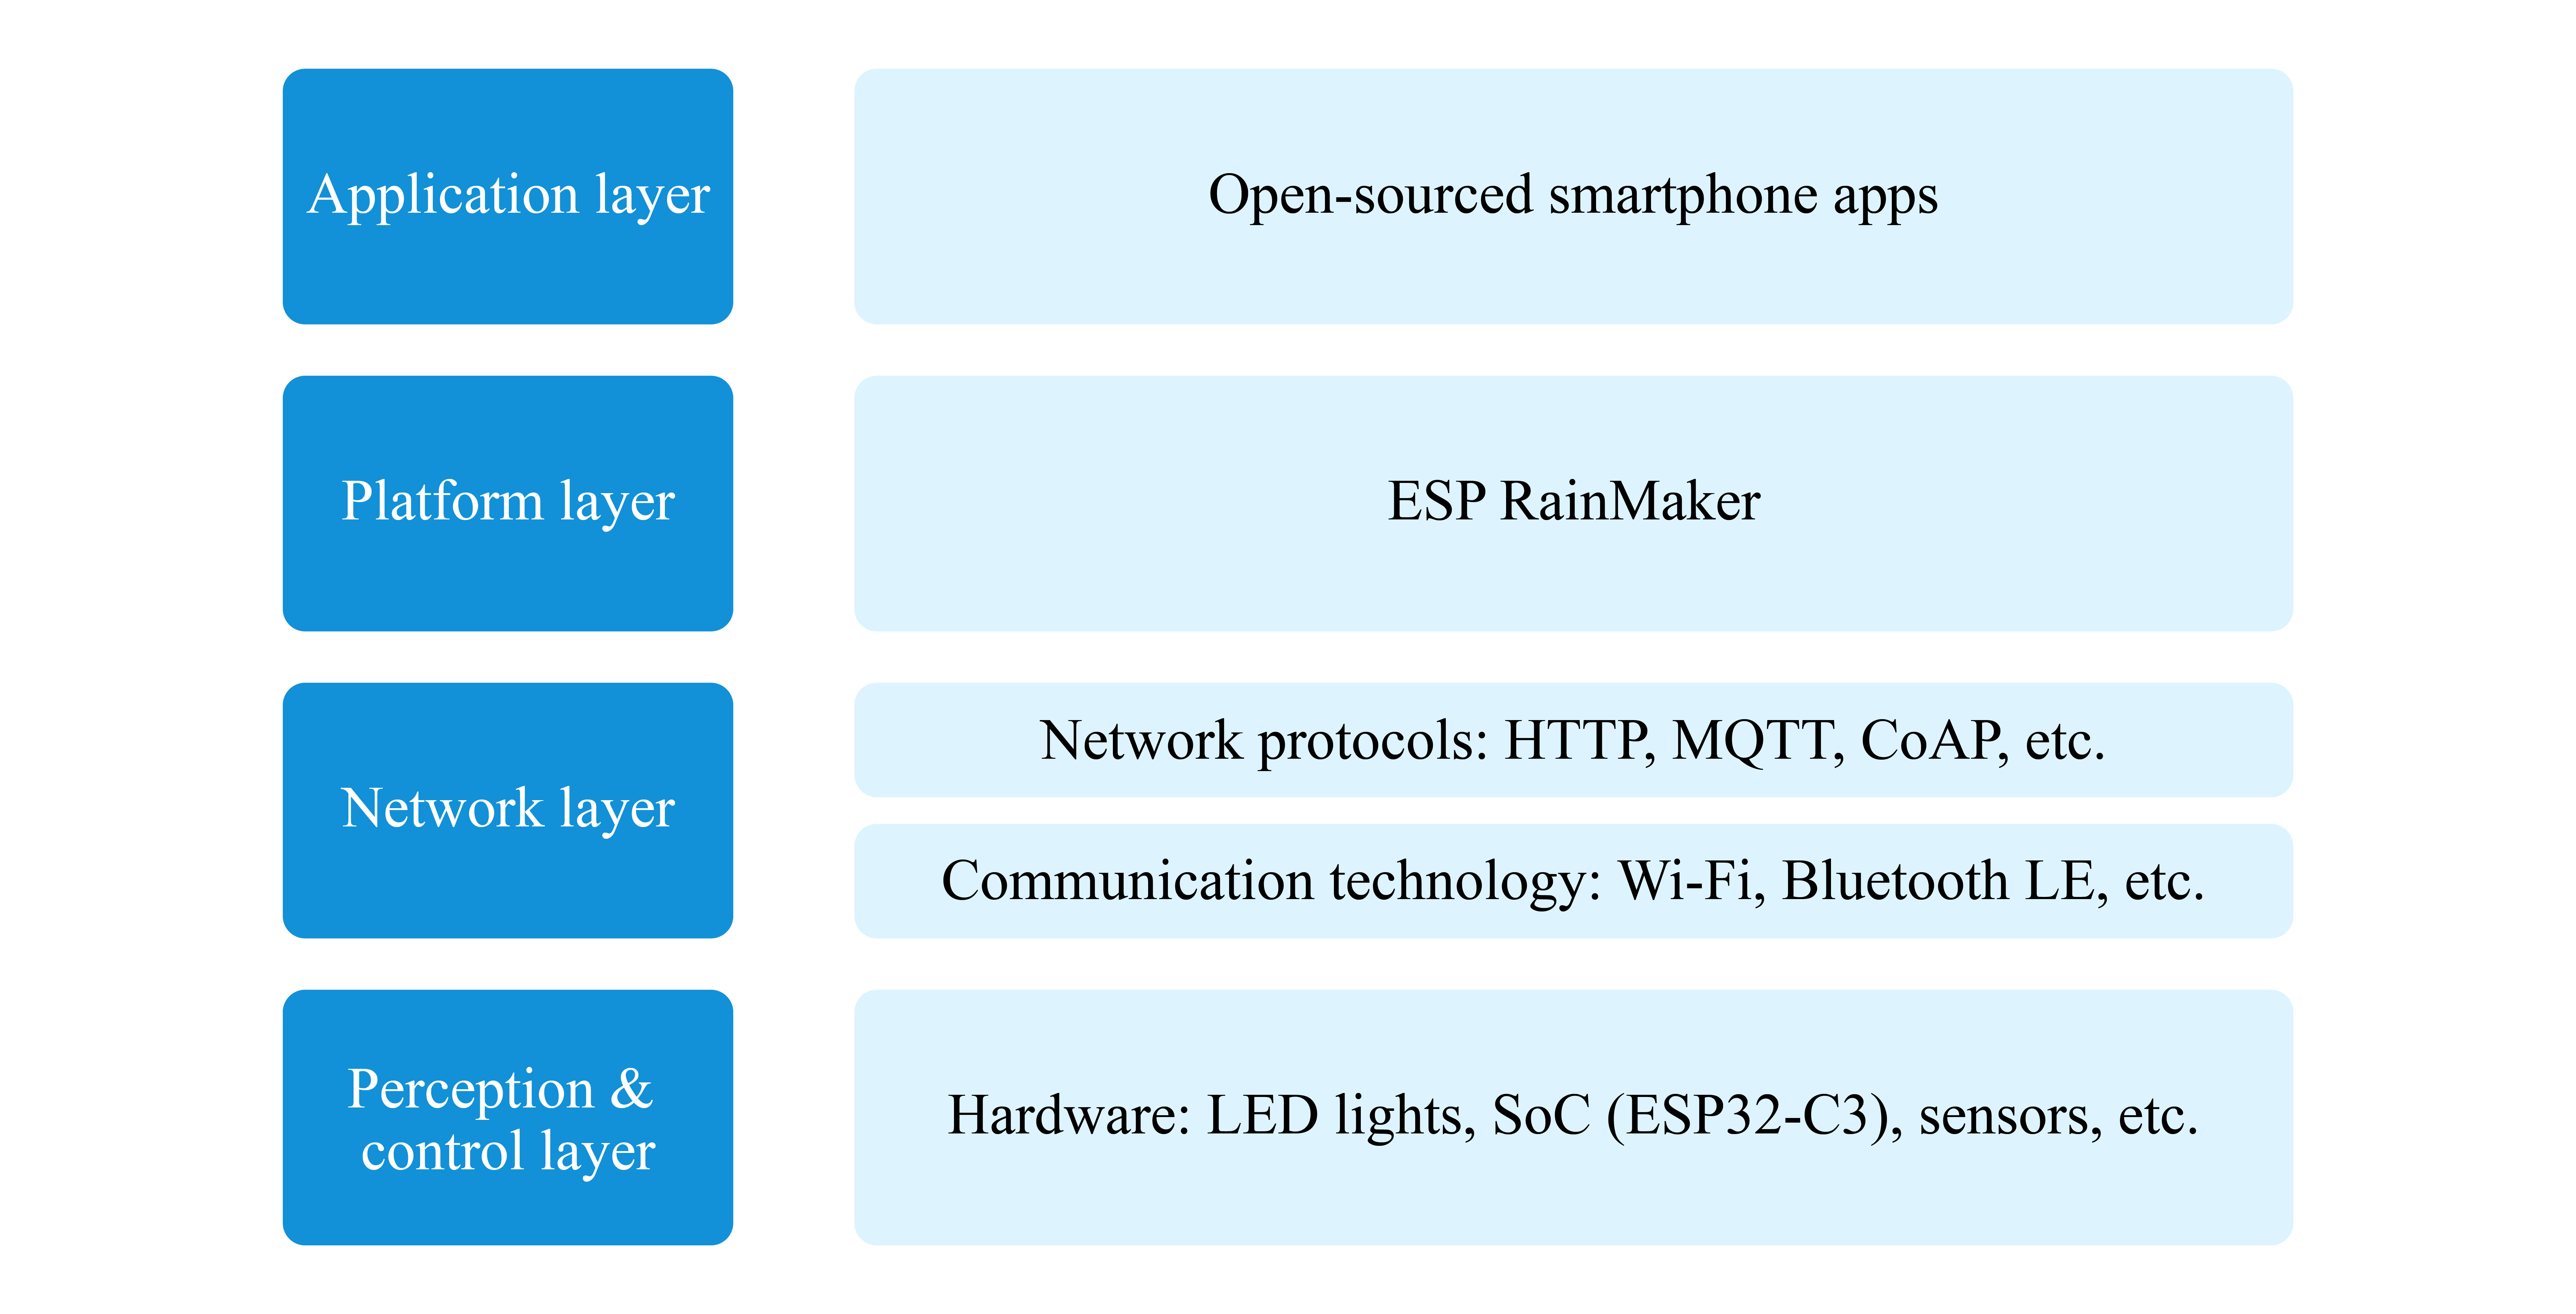
\includegraphics[width=0.7\textwidth]{D2Z/2-1}
    \caption{Structure of smart light project}
\end{figure}

\subsection{Project Functions}
Divided according to the structure, functions of each part are as follows.

\begin{term}{Smart light devices}
    \begin{itemize}
        \item Network configuration and connection.
        \item LED PWM control, such as switch, brightness, color temperature, etc.
        \item Automation or scene control, e.g., time switch.
        \item Encryption and secure boot of the Flash.
        \item Firmware upgrade and version management.
    \end{itemize}
\end{term}

\begin{term}{Smartphone apps}
    \begin{itemize}
        \item Network configuration and device binding.
        \item Smart light product control, such as switch, brightness, color temperature, etc.
        \item Automation or scene settings, e.g., time switch.
        \item Local/remote control.
        \item User registration, login, etc.
    \end{itemize}
\end{term}

\begin{term}{ESP RainMaker IoT cloud platform}
    \begin{itemize}
        \item Enabling IoT device access.
        \item Providing device operation APIs accessible to smartphone apps.
        \item Firmware upgrade and version management.
    \end{itemize}
\end{term}

\subsection{Hardware Preparation}
If interested in putting the project into practice, you will also need the following hardware: smart lights, smartphones, Wi-Fi routers, and a computer that meets the installation requirements of the development environment.

\begin{term}{Smart lights}
    Smart lights are a new type of bulbs, whose shape is the same as the general incandescent bulb. A smart light is composed of capacitor step-down regulated power supply, wireless module (with built-in ESP32-C3), LED controller and RGB LED matrix. When connected to power, the 15 V DC voltage output after capacitor step-down, diode rectification, and regulation provides energy to the LED controller and LED matrix. The LED controller can automatically send high and low levels at certain intervals, switching the RGB LED matrix between closed (lights on) and open (lights off), so that it can emit cyan, yellow, green, purple, blue, red, and white light. The wireless module is responsible for connecting to the Wi-Fi router, receiving and reporting the status of smart lights, and sending commands to control the LED.

    \begin{figure}[!ht]
        \centering
        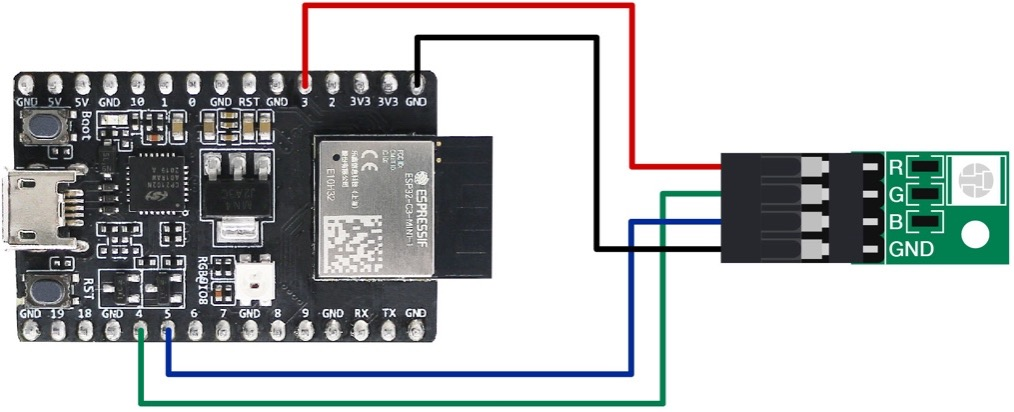
\includegraphics[width=0.6\textwidth]{D2Z/2-2}
        \caption{A simulated smart light}
    \end{figure}

    In the early development stage, you can simulate a smart light using the ESP32-C3-DevKitM-1 board connected with RGB LED lamp beads (see Figure 2.2). But you should note that this is not the only way to assemble a smart light. The hardware design of the project in this book only contains a wireless module (with built-in ESP32-C3), but not a complete smart light hardware design.

    \parskip 6pt
    In addition, Espressif also produces a ESP32-C3-based audio development board – ESP32-C3-Lyra – for controlling lights with audio. The board has interfaces for microphones and speakers and can control LED strips. It can be used for developing ultra-low-cost, high-performance audio broadcasters and rhythm light strips. Figure 2.3 shows a ESP32-C3-Lyra board linked with a strip of 40 LED lights.

    \begin{figure}[!ht]
        \centering
        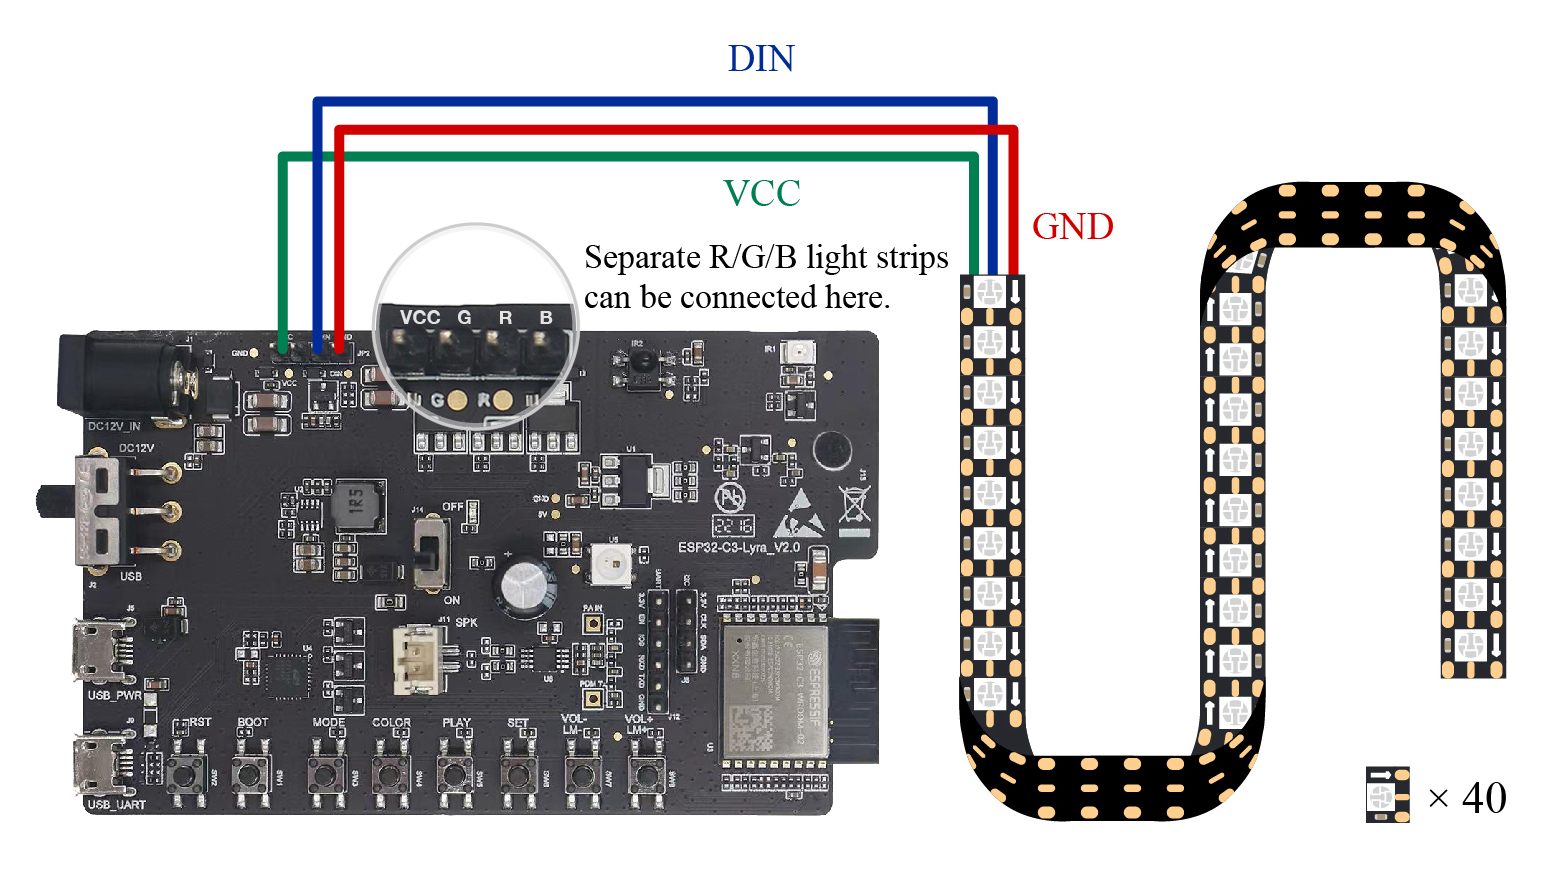
\includegraphics[width=0.75\textwidth]{D2Z/2-3}
        \caption{ESP32-C3-Lyra linked with a strip of 40 LED lights}
    \end{figure}
\end{term}

\begin{term}{Smartphones (Android/iOS)}
    The Smart Light project involves the development of a smartphone app for setting up and controlling smart light products.
\end{term}

\begin{term}{Wi-Fi routers}
    Wi-Fi routers convert wired network signals and mobile network signals into wireless network signals, for computers, smartphones, tablets, and other wireless devices to connect to the network. For example, broadband in the home only needs to be connected to a Wi-Fi router to achieve wireless networking of Wi-Fi devices. The mainstream protocol standard supported by Wi-Fi routers is IEEE 802.11n, with an average TxRate of 300 Mbps, or 600 Mbps at maximum. They are backward compatible with IEEE 802.11b and IEEE 802.11g. The ESP32-C3 chip by Espressif supports IEEE 802.11b/g/n, so you can choose a single-band (2.4 GHz) or dual-band (2.4 GHz and 5 GHz) Wi-Fi router.
\end{term}

\begin{term}{A computer (Linux/macOS/Windows)}
    Development environment will be introduced in Chapter 4.
\end{term}

\subsection{Development Process}
\begin{figure}[!ht]
        \centering
        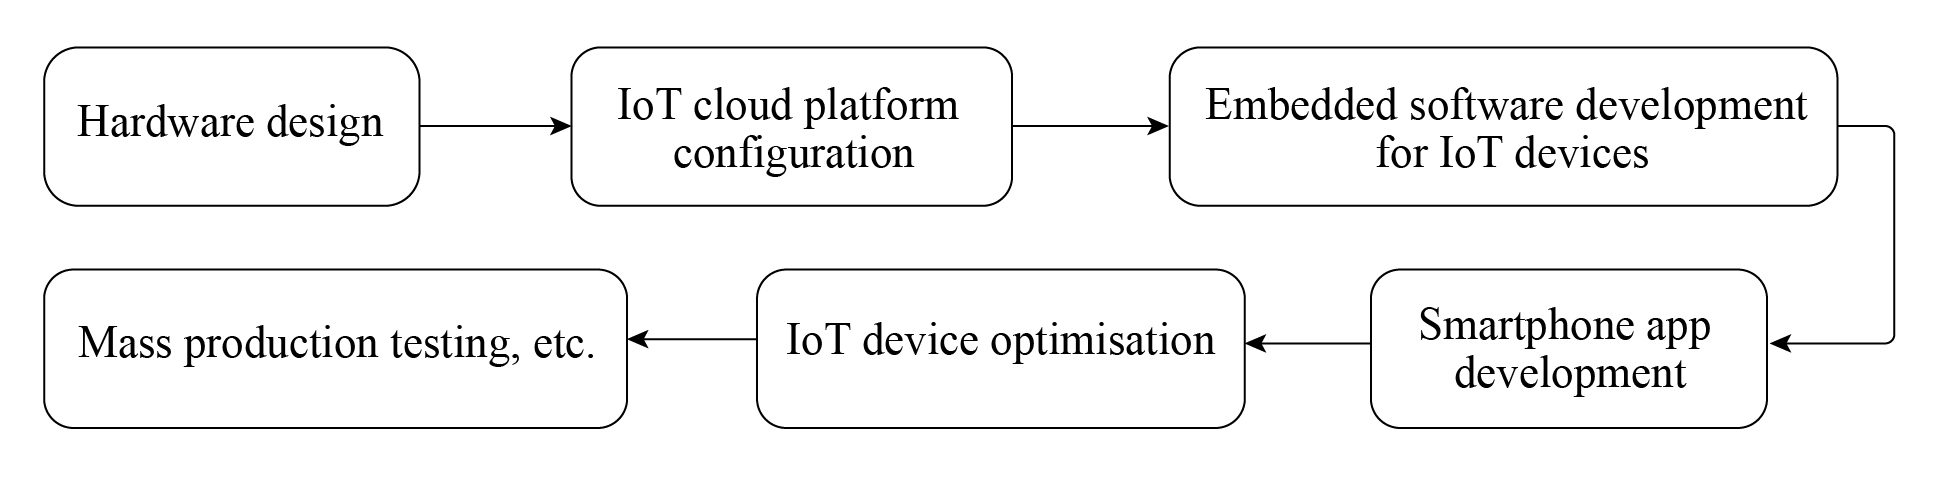
\includegraphics[width=0.8\textwidth]{D2Z/2-4}
        \caption{Steps of developing the Smart Light project}
\end{figure}

\begin{term}{Hardware design}
    Hardware design of IoT devices is essential to an IoT project. A complete smart light project is intended to produce a lamp working under mains supply. Different manufacturers produce lamps of different styles and driver types, but their wireless modules are usually of the same function. To simplify the development process of the Smart Ligh project, this book only covers the hardware design and software development of wireless modules.
\end{term}

\begin{term}{IoT cloud platform configuration}
    To use IoT cloud platforms, you need to configure projects on the backend, such as creating products, creating devices, setting device properties, etc.
\end{term}

\begin{term}{Embedded software development for IoT devices}
    Implement expected functions with ESP-IDF, Espressif’s device-side SDK, including connecting to IoT cloud platforms, developing LED drivers, and upgrading firmware.
\end{term}

\begin{term}{Smartphone app development}
    Develop smartphone apps for Android and iOS systems to realise user registration and login, device control and other functions.
\end{term}

\begin{term}{IoT device optimisation}
    Once the basic development of IoT device functions is completed, you may turn to optimisation tasks, such as power optimisation.
\end{term}

\begin{term}{Mass production testing}
    Carry out mass production tests according to related standards, such as equipment function test, aging test, RF test, etc.
\end{term}

Despite the steps listed above, a Smart Light project is not necessarily subject to such procedure as different tasks can also be carried out at the same time. For example, embedded software and smartphone apps can be developed in parallel. Some steps may also need to be repeated, such as IoT device optimisation and mass production testing.

\section{Summary}
In this chapter, we first expounded on the basic components and functional modules of an IoT project, then introduced the Smart Light case for practice, refering to its structure, functions, hardware preparation, and development process. Readers can draw inferences from the practice and become confident to carry out IoT projects with minimum mistakes in the future.

\end{document}
